% \begin{figure}[htbp]
%     \centering
%     \includegraphics[width=0.48\textwidth]{figures/rw_task_figure.pdf}
%     \caption{Visualization of real-world tasks.}
%     \label{fig:pull_figure}
% \end{figure}

\begin{figure*}[t]
    % \vspace{0.5cm}
    \centering
    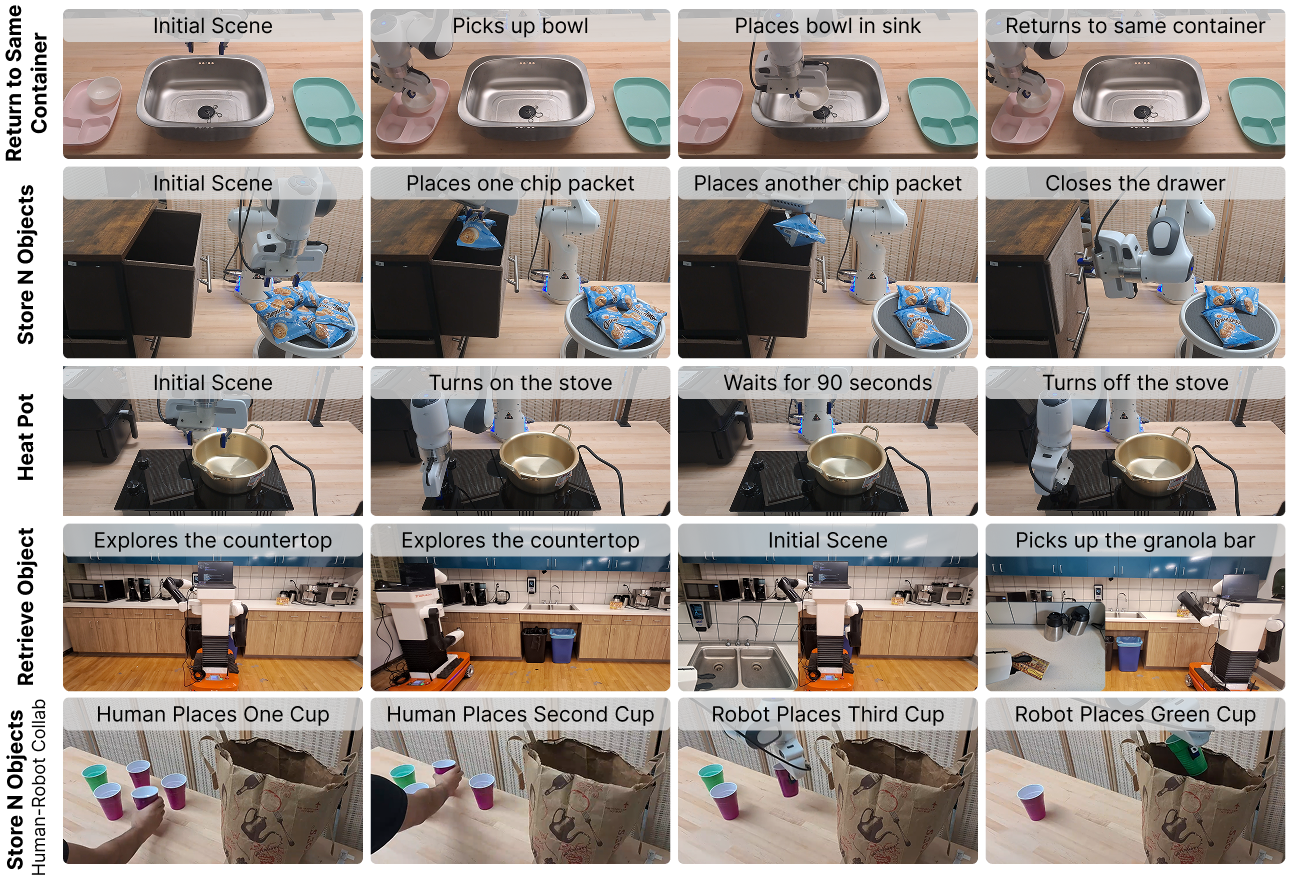
\includegraphics[width=0.98\textwidth]{figures/rw_task_figure_5.png}
    \vspace{-10pt}
    \caption{\textbf{Visualization of real-world tasks.} We evaluate \ourmethod{} in four stationary and mobile manipulation tasks, including a human-robot collaborative task (\textit{rows}) with strong partial observability, where the agent needs to retrieve different types of information from memory. The pictures in each column depict a different phase of the task.}
    \label{fig:rw_task_viz}
    \vspace{-10pt}
\end{figure*}
